% Scaling circles S_r and the ripple pencil C_t = J(Hhat_t).
\documentclass[tikz,border=8pt]{standalone}
\usepackage{amsmath,amssymb}
\begin{document}
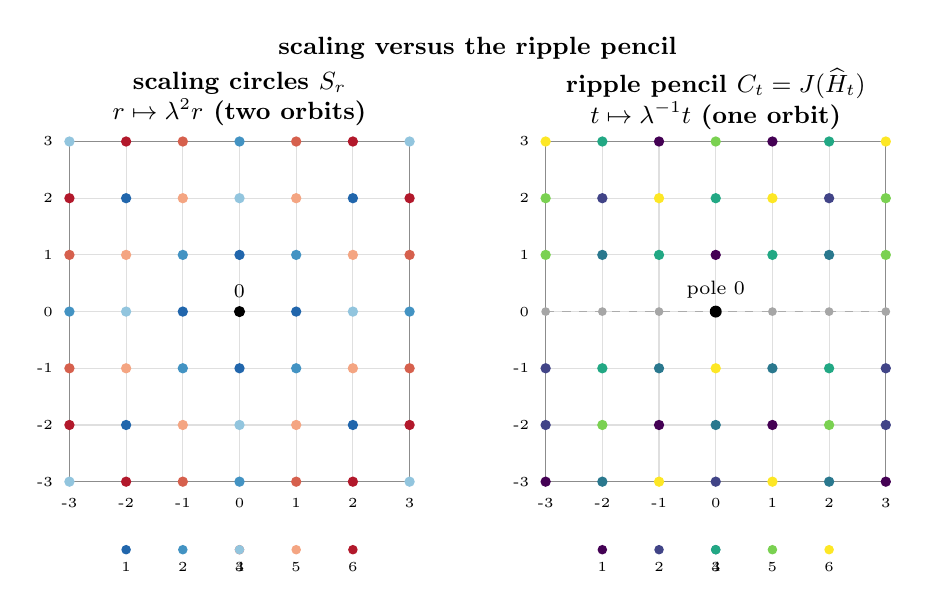
\begin{tikzpicture}[scale=0.72]
% colours: squares 1,2,4 in blue; nonsquares 3,5,6 in red/orange
\definecolor{sA}{HTML}{2166AC}
\definecolor{sB}{HTML}{4393C3}
\definecolor{sC}{HTML}{D6604D}
\definecolor{sD}{HTML}{92C5DE}
\definecolor{sE}{HTML}{F4A582}
\definecolor{sF}{HTML}{B2182B}
\definecolor{tA}{HTML}{440154}
\definecolor{tB}{HTML}{414487}
\definecolor{tC}{HTML}{2A788E}
\definecolor{tD}{HTML}{22A884}
\definecolor{tE}{HTML}{7AD151}
\definecolor{tF}{HTML}{FDE725}
\begin{scope}[xshift=-4.2cm]
  \draw[gray!25] (-3,-3) grid (3,3);
  \draw[black!45] (-3,-3) rectangle (3,3);
  \foreach \x in {-3,...,3} {\node[font=\tiny,below] at (\x,-3.12) {\x};}
  \foreach \y in {-3,...,3} {\node[font=\tiny,left] at (-3.12,\y) {\y};}
  \fill[sA] (-2,-2) circle (2.6pt);
  \fill[sA] (-2,2) circle (2.6pt);
  \fill[sA] (-1,0) circle (2.6pt);
  \fill[sA] (0,-1) circle (2.6pt);
  \fill[sA] (0,1) circle (2.6pt);
  \fill[sA] (1,0) circle (2.6pt);
  \fill[sA] (2,-2) circle (2.6pt);
  \fill[sA] (2,2) circle (2.6pt);
  \fill[sB] (-3,0) circle (2.6pt);
  \fill[sB] (-1,-1) circle (2.6pt);
  \fill[sB] (-1,1) circle (2.6pt);
  \fill[sB] (0,-3) circle (2.6pt);
  \fill[sB] (0,3) circle (2.6pt);
  \fill[sB] (1,-1) circle (2.6pt);
  \fill[sB] (1,1) circle (2.6pt);
  \fill[sB] (3,0) circle (2.6pt);
  \fill[sC] (-3,-1) circle (2.6pt);
  \fill[sC] (-3,1) circle (2.6pt);
  \fill[sC] (-1,-3) circle (2.6pt);
  \fill[sC] (-1,3) circle (2.6pt);
  \fill[sC] (1,-3) circle (2.6pt);
  \fill[sC] (1,3) circle (2.6pt);
  \fill[sC] (3,-1) circle (2.6pt);
  \fill[sC] (3,1) circle (2.6pt);
  \fill[sD] (-3,-3) circle (2.6pt);
  \fill[sD] (-3,3) circle (2.6pt);
  \fill[sD] (-2,0) circle (2.6pt);
  \fill[sD] (0,-2) circle (2.6pt);
  \fill[sD] (0,2) circle (2.6pt);
  \fill[sD] (2,0) circle (2.6pt);
  \fill[sD] (3,-3) circle (2.6pt);
  \fill[sD] (3,3) circle (2.6pt);
  \fill[sE] (-2,-1) circle (2.6pt);
  \fill[sE] (-2,1) circle (2.6pt);
  \fill[sE] (-1,-2) circle (2.6pt);
  \fill[sE] (-1,2) circle (2.6pt);
  \fill[sE] (1,-2) circle (2.6pt);
  \fill[sE] (1,2) circle (2.6pt);
  \fill[sE] (2,-1) circle (2.6pt);
  \fill[sE] (2,1) circle (2.6pt);
  \fill[sF] (-3,-2) circle (2.6pt);
  \fill[sF] (-3,2) circle (2.6pt);
  \fill[sF] (-2,-3) circle (2.6pt);
  \fill[sF] (-2,3) circle (2.6pt);
  \fill[sF] (2,-3) circle (2.6pt);
  \fill[sF] (2,3) circle (2.6pt);
  \fill[sF] (3,-2) circle (2.6pt);
  \fill[sF] (3,2) circle (2.6pt);
  \fill[black] (0,0) circle (2.8pt);
  \node[font=\scriptsize] at (0,0.35) {$0$};
  \node[font=\small\bfseries,align=center] at (0,3.75) {scaling circles $S_r$\\ $r\mapsto\lambda^2r$ (two orbits)};
  \fill[sA] (-2,-4.2) circle (2.4pt);
  \node[font=\tiny,below] at (-2,-4.25) {$1$};
  \fill[sB] (-1,-4.2) circle (2.4pt);
  \node[font=\tiny,below] at (-1,-4.25) {$2$};
  \fill[sC] (0,-4.2) circle (2.4pt);
  \node[font=\tiny,below] at (0,-4.25) {$3$};
  \fill[sD] (0,-4.2) circle (2.4pt);
  \node[font=\tiny,below] at (0,-4.25) {$4$};
  \fill[sE] (1,-4.2) circle (2.4pt);
  \node[font=\tiny,below] at (1,-4.25) {$5$};
  \fill[sF] (2,-4.2) circle (2.4pt);
  \node[font=\tiny,below] at (2,-4.25) {$6$};
\end{scope}
\begin{scope}[xshift=4.2cm]
  \draw[gray!25] (-3,-3) grid (3,3);
  \draw[black!45] (-3,-3) rectangle (3,3);
  \foreach \x in {-3,...,3} {\node[font=\tiny,below] at (\x,-3.12) {\x};}
  \foreach \y in {-3,...,3} {\node[font=\tiny,left] at (-3.12,\y) {\y};}
  \fill[tA] (-3,-3) circle (2.6pt);
  \fill[tA] (-1,-2) circle (2.6pt);
  \fill[tA] (-1,3) circle (2.6pt);
  \fill[tA] (0,1) circle (2.6pt);
  \fill[tA] (1,-2) circle (2.6pt);
  \fill[tA] (1,3) circle (2.6pt);
  \fill[tA] (3,-3) circle (2.6pt);
  \fill[tB] (-3,-2) circle (2.6pt);
  \fill[tB] (-3,-1) circle (2.6pt);
  \fill[tB] (-2,2) circle (2.6pt);
  \fill[tB] (0,-3) circle (2.6pt);
  \fill[tB] (2,2) circle (2.6pt);
  \fill[tB] (3,-2) circle (2.6pt);
  \fill[tB] (3,-1) circle (2.6pt);
  \fill[tC] (-2,-3) circle (2.6pt);
  \fill[tC] (-2,1) circle (2.6pt);
  \fill[tC] (-1,-1) circle (2.6pt);
  \fill[tC] (0,-2) circle (2.6pt);
  \fill[tC] (1,-1) circle (2.6pt);
  \fill[tC] (2,-3) circle (2.6pt);
  \fill[tC] (2,1) circle (2.6pt);
  \fill[tD] (-2,-1) circle (2.6pt);
  \fill[tD] (-2,3) circle (2.6pt);
  \fill[tD] (-1,1) circle (2.6pt);
  \fill[tD] (0,2) circle (2.6pt);
  \fill[tD] (1,1) circle (2.6pt);
  \fill[tD] (2,-1) circle (2.6pt);
  \fill[tD] (2,3) circle (2.6pt);
  \fill[tE] (-3,1) circle (2.6pt);
  \fill[tE] (-3,2) circle (2.6pt);
  \fill[tE] (-2,-2) circle (2.6pt);
  \fill[tE] (0,3) circle (2.6pt);
  \fill[tE] (2,-2) circle (2.6pt);
  \fill[tE] (3,1) circle (2.6pt);
  \fill[tE] (3,2) circle (2.6pt);
  \fill[tF] (-3,3) circle (2.6pt);
  \fill[tF] (-1,-3) circle (2.6pt);
  \fill[tF] (-1,2) circle (2.6pt);
  \fill[tF] (0,-1) circle (2.6pt);
  \fill[tF] (1,-3) circle (2.6pt);
  \fill[tF] (1,2) circle (2.6pt);
  \fill[tF] (3,3) circle (2.6pt);
  \draw[gray!65, dashed] (-3,0)--(3,0);
  \fill[gray!70] (-3,0) circle (2.2pt);
  \fill[gray!70] (-2,0) circle (2.2pt);
  \fill[gray!70] (-1,0) circle (2.2pt);
  \fill[gray!70] (1,0) circle (2.2pt);
  \fill[gray!70] (2,0) circle (2.2pt);
  \fill[gray!70] (3,0) circle (2.2pt);
  \fill[black] (0,0) circle (3.0pt);
  \node[font=\scriptsize] at (0.0,0.38) {pole $0$};
  \node[font=\small\bfseries,align=center] at (0,3.75) {ripple pencil $C_t=J(\widehat H_t)$\\ $t\mapsto\lambda^{-1}t$ (one orbit)};
  \fill[tA] (-2,-4.2) circle (2.4pt);
  \node[font=\tiny,below] at (-2,-4.25) {$1$};
  \fill[tB] (-1,-4.2) circle (2.4pt);
  \node[font=\tiny,below] at (-1,-4.25) {$2$};
  \fill[tC] (0,-4.2) circle (2.4pt);
  \node[font=\tiny,below] at (0,-4.25) {$3$};
  \fill[tD] (0,-4.2) circle (2.4pt);
  \node[font=\tiny,below] at (0,-4.25) {$4$};
  \fill[tE] (1,-4.2) circle (2.4pt);
  \node[font=\tiny,below] at (1,-4.25) {$5$};
  \fill[tF] (2,-4.2) circle (2.4pt);
  \node[font=\tiny,below] at (2,-4.25) {$6$};
\end{scope}
\node[font=\small\bfseries] at (0,4.65) {scaling versus the ripple pencil};
\end{tikzpicture}
\end{document}